\subsubsection{Reificazione dei generics}
La reificazione delle definizioni generiche è responsabilità della classe \texttt{GenericsInstantiationEngine}. Di essa 
si crea un'istanza per ogni definizione che si desidera istanziare, costruendola a partire dalle regole di istanziazione, ovvero 
una struttura dati che tiene traccia di quale parametro attuale di tipo corrisponda a quale tipo generico. La reificazione 
avviene mediante \textit{match-and-replace} (rimpiazzamento).  \\

\begin{figure}[H]
    \centering
        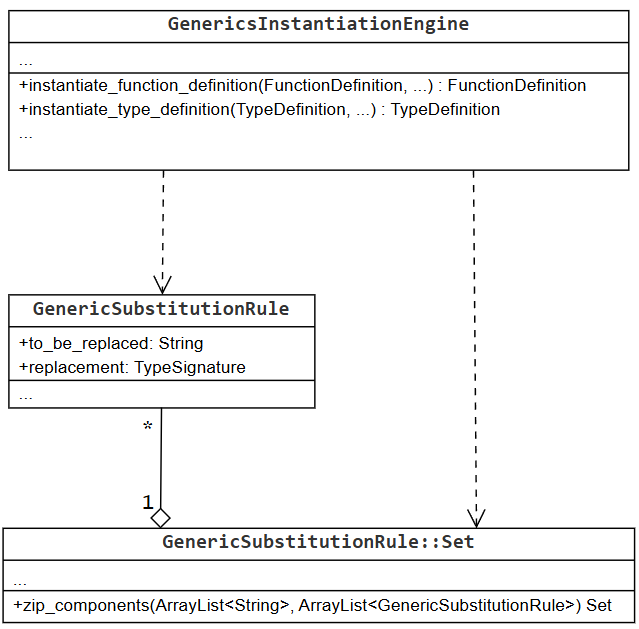
\includegraphics[scale=0.7]{../../Assets/GenericsUML.png}
    \caption{Diagramma UML delle classi che concorrono alla reificazione dei generics}
\end{figure}

\newpage

L'implementazione di tale classe è abbastanza semplice, in quanto si limita a visitare ricorsivamente i nodi dell'AST 
dell'oggetto da istanziare, mediante visita in profondità (DFS), rimpiazzando i tipi generici con i tipi concreti 
qualora essa li incontra. \\

\vspace{0.5cm}
\begin{lstlisting}[frame=single]
class GenericsInstantiationEngine {

    public:
        GenericsInstantiationEngine(GenericSubstitutionRule::Set&);

        TypeSignature instantiate_generic_type(TypeSignature&);
       
        Statement instantiate_generic_statement(Statement&);
                
        Expression instantiate_generic_expression(Expression&);
        
        TypeDefinition instantiate_generic_typedefinition(
            TypeDefinition& type_signature,
            string& new_type_name
        );
        
        FunctionDefinition::Ref instantiate_generic_function(
            FunctionDefinition& function_definition,
            string& new_function_name
        );

        FunctionDefinition::Ref instantiate_generic_function(
            FunctionDefinition& function_definition_ref, 
            string& new_function_name
        );

        /* other methods */

    private:
        GenericSubstitutionRule::Set rules;
};
\end{lstlisting}
\vspace{0.5cm}

Per reificare (istanziare) una definizione, è necessario fornire un nuovo nome da dargli, in quanto 
due definizioni non possono avere lo stesso nome. All'interno della funzione generica istanziata 
si vanno a inserire i nomi completi dei tipi concreti al posto del numero di generics 
(si faccia riferimento al formato di indicizzazione delle definizioni nelle varie tabelle). \\

\newpage